\begin{comment}
	Split data according to percentile
	RFCN resnet-101
	Pascal voc heavily skewed to smaller objects. Show plot
	50th percentile 13892.0
\end{comment}

\section{Resolution-Aware Object Detection}
Object detectors are commonly more accurate on objects that cover a larger number of pixels in an image. This is intuitive as objects with a lower resolution objectively have less details that can describe them. The poorer performance can be seen in \tableref{cocores}, for all object detectors the \gls{ap} is considerably lower for smaller objects in comparison to both medium and large. The best performing detector from \cite{deepres}, has an \gls{ap} difference of 35.3\%, from 50.9\% for large objects to 15.6\% for small. 
A potential method of tackling this issue is to train multiple detectors on separate partitions of the training data according to the size of the object. While deep-based \gls{cnn} have millions of parameters to generalise from training to testing, the difference between small and large objects may skew the learning towards the latter. In order to test this hypothesis an initial test will be conducted on the \gls{pascalvoc} dataset. However, \gls{pascalvoc} does not have the same definition of objects sizes as in \gls{mscoco}. Therefore, the distribution of the bounding boxes from the training set must be analysed in order to determine an appropriate split of data based on object size. This was done by parsing all of the bounding box coordinates in the 07++12 training set and calculating the area. A histogram of the area can be seen in \figref{0712hist}. There is a clear tendency to smaller objects in the training set with a clear skew towards the left of the figure.

\begin{figure}[H]
  \centering
    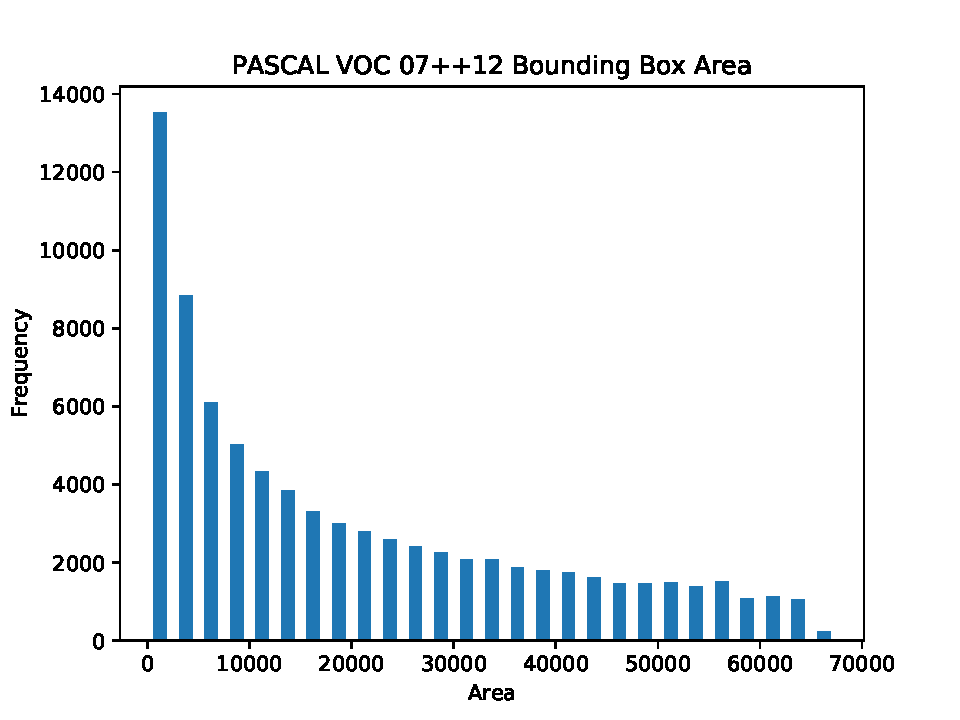
\includegraphics[width=0.6\textwidth]{Figs/Implementation/0712hist.pdf}
      \caption{Histogram of the \gls{pascalvoc} 07++12 bounding box area.}
    \label{fig:0712hist}
\end{figure}

As there is no clear way to split the data into three sets with equal amounts of data it was instead split into two sets, one for small objects and another for larger. The split was made at the median area which is 13,892 pixels. Therefore, the dataset with area less than 13,982 pixels is denoted 07++12$_{small}$ and objects larger make up the dataset 07++12$_{larger}$.

